% Figure 5: the six recorded paired cluster-bootstrap differences between fine-tuned models.
% source: H8b primary and should-decline rows, docs/experiments.md (EXP:545-549, 564):
%   answerable -0.0168 [-0.0546, +0.0177]; should-decline -0.0111 [-0.0429, +0.0195].
% source: H9 primary row (EXP:748-752) and should-decline row (EXP:768-770; L2:166):
%   answerable +0.0409 [+0.0040, +0.0780]; should-decline +0.1020 [-0.0018, +0.2062].
% source: Logos v0.0.1 -> v0.0.2, Logos v0.0.2 report section 8 (L2:204-210):
%   answerable +0.0577 [+0.0234, +0.0952]; should-decline +0.1131 [+0.0028, +0.2296].
% Answerable rows resample 61 groups, should-decline rows 17. Error-bar lengths are the
% distances from each estimate to its recorded interval endpoints.
\begin{figure}[t]
\centering
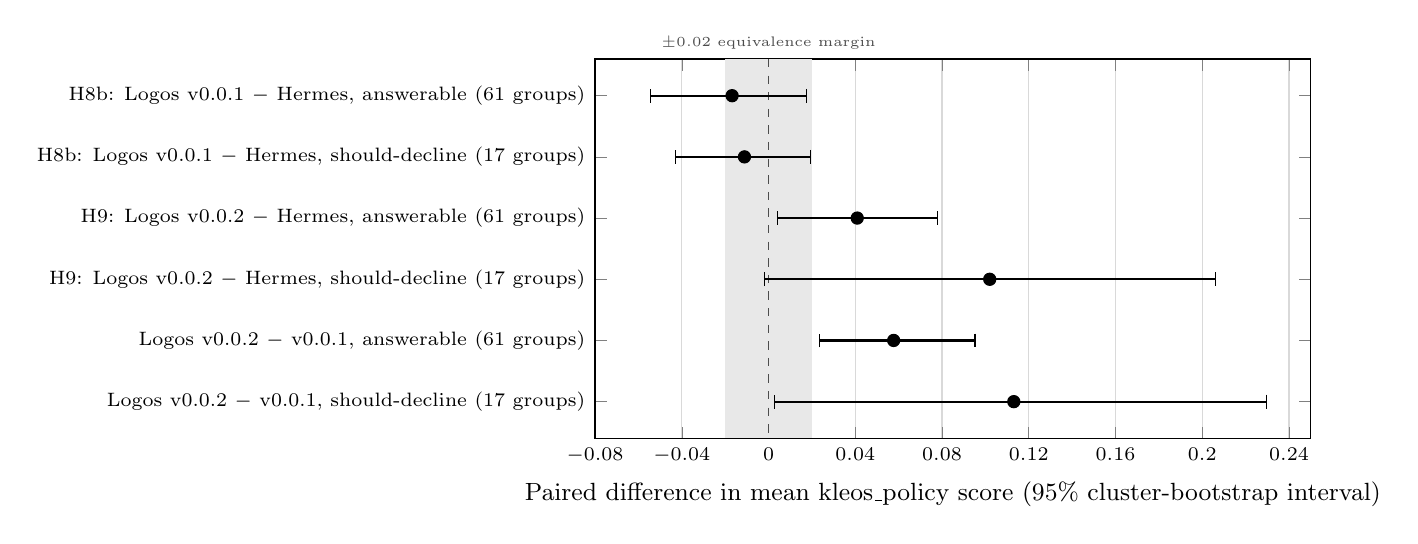
\begin{tikzpicture}
\begin{axis}[
  width=0.88\linewidth, height=6.4cm,
  xlabel={Paired difference in mean \code{kleos\_policy} score (95\% cluster-bootstrap interval)},
  xmin=-0.08, xmax=0.25,
  xtick={-0.08,-0.04,0,0.04,0.08,0.12,0.16,0.20,0.24},
  scaled x ticks=false, xticklabel style={/pgf/number format/fixed, /pgf/number format/precision=2},
  ymin=0.4, ymax=6.6, y dir=reverse,
  ytick={1,2,3,4,5,6},
  yticklabels={
    {H8b: Logos v0.0.1 $-$ Hermes, answerable (61 groups)},
    {H8b: Logos v0.0.1 $-$ Hermes, should-decline (17 groups)},
    {H9: Logos v0.0.2 $-$ Hermes, answerable (61 groups)},
    {H9: Logos v0.0.2 $-$ Hermes, should-decline (17 groups)},
    {Logos v0.0.2 $-$ v0.0.1, answerable (61 groups)},
    {Logos v0.0.2 $-$ v0.0.1, should-decline (17 groups)}},
  y tick label style={font=\scriptsize, align=right},
  tick label style={font=\scriptsize}, label style={font=\small},
  xmajorgrids, grid style={gray!30},
  clip=false,
]
\fill[gray!18] (axis cs:-0.02,0.4) rectangle (axis cs:0.02,6.6);
\draw[dashed, gray!60!black] (axis cs:0,0.4) -- (axis cs:0,6.6);
\node[font=\tiny, gray!60!black, anchor=south] at (axis cs:0,0.4) {$\pm 0.02$ equivalence margin};
\addplot[only marks, mark=*, mark size=2.2pt, color=black,
  error bars/.cd, x dir=both, x explicit, error bar style={thick}, error mark options={rotate=90, mark size=2.5pt}]
  table[x=est, y=row, x error plus=ep, x error minus=em] {
est row ep em
-0.0168 1 0.0345 0.0378
-0.0111 2 0.0306 0.0318
0.0409 3 0.0371 0.0369
0.1020 4 0.1042 0.1038
0.0577 5 0.0375 0.0343
0.1131 6 0.1165 0.1103
};
\end{axis}
\end{tikzpicture}
\caption{Paired differences between fine-tuned models, resampled by benchmark group (2,000 resamples). The primary rows are the answerable ones: H8b is inconclusive because its interval crosses zero and is not contained in the $\pm 0.02$ equivalence margin, and H9 is ``better'' because its interval lies entirely above zero. The should-decline rows rest on 17 groups; only the v0.0.1 to v0.0.2 row excludes zero.}
\label{fig:forest}
\end{figure}
